\subsection{Fourth-Order Runge-Kutta Method}\label{sec:rk4}
The Runge-Kutta methods can be understood as an improvement of Euler's method. The most used order for Runge-Kutta methods is four, since for lower orders, the method is not accurate enough, and for higher orders, the method does not provide significant improvements in the approximations \cite{mathews2004numerical}.

The fourth-order Runge-Kutta (RK4) method is given by
\begin{equation}
    y _ { i + 1 } = y _ { i } + h\left(\dfrac{k_1+2k_2+2k_3+k_4}{6}\right)
\end{equation}
where 
\begin{equation*}
    \begin{array} { l } { k _ { 1 } = f \left( t _ { i } , y _ { i } \right) } \\
    { k _ { 2 } = f \left( t _ { i } + h / 2 , y _ { i } + h k _ { 1 } / 2 \right) } \\
    { k _ { 3 } = f \left( t _ { i } + h / 2 , y _ { i } + h k _ { 2 } / 2 \right) } \\ 
    { k _ { 4 } = f \left( t _ { i } + h , y _ { i } + h k _ { 3 } \right) } \end{array}
\end{equation*}

\subsubsection{Visualization}
This section is inspired and adapted on the explanation presented in \cite{vis_rk4}. Figure \ref{fig:RK4Visual} shows how RK4 works. It calculates four different slopes based on the previous one and then it takes the average of this slopes for a better accuracy. 

The method takes the slope at time $t=t_0$, for example, and then it makes an approximation just as Euler's method ($k_1$) until $t_1$, then it looks for the slope ($k_2$) in half that time through the same $y$ approximation as $k_1$; then, it looks for the half the change of $y$ then looks for the slope ($k_3)$ in the same time with this new $y$ value. Finally, it repeats this procedure in order to find the last slope ($k_4$).

Notice that this method includes the rate of change of the function between the time steps and after it, in order to calculate a more accurate slope and use it for the new approximation.

\begin{figure}[H]
    \centering
    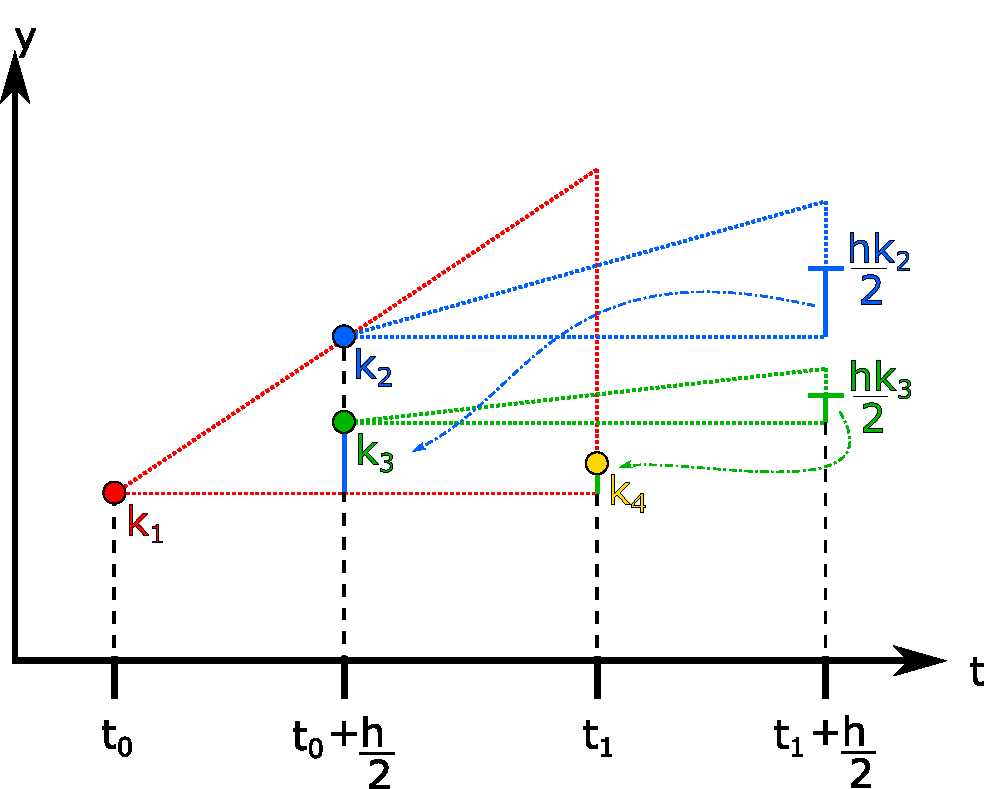
\includegraphics[scale=0.4]{files/sv.pdf}
    \caption{RK4 visualization.}
    \label{fig:RK4Visual}
\end{figure}


\begin{exmp}
Solve the following initial value problem using RK4 method \cite{exampleeuler}.
\begin{equation}
\begin{cases}
    y'+2y=2-e^{-4t}&\\ y(0)=1\quad t\in[0,2.5]& 
\end{cases}
\end{equation}
\end{exmp}
Notice that is the same  problem as the example \ref{ex:r_e}, where is shown the exact solution.
\begin{figure}[H]
    \centering
    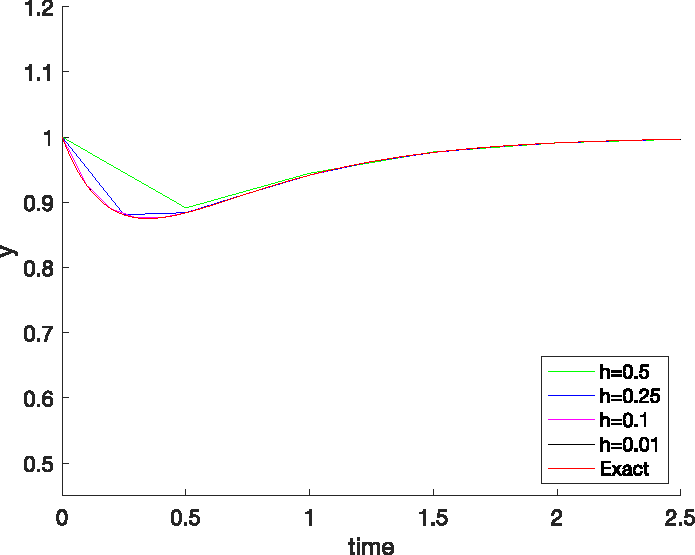
\includegraphics[scale=0.5]{files/exampleKutta.pdf}
    \caption{Results for smaller step sizes using RK4.}
    \label{fig:exkutta}
\end{figure}

In order to compare with the results obtained in section \ref{sec:euler}, let us use the same example.
\begin{exmp}
Solve the following initial value problem using RK4 method \cite{exampleeuler}.
\begin{equation}
\begin{cases}
    y'-y=-\dfrac{1}{2}e^{\frac{t}{2}}\sin(5t)+5e^{\frac{t}{2}}\cos(5t)&\\y(0)=0\quad t\in[0,7.5]&
    \end{cases}
\end{equation}\label{eq:ex2kutta}
\end{exmp}

\begin{table}[H]
\centering
\begin{tabular}{cccccc}
\hline
\textbf{Time}           & \textbf{\boldmath$h=0.5$} & \textbf{\boldmath$h=0.25$} & \textbf{\boldmath$h=0.1$} & \textbf{\boldmath$h=0.01$} & \textbf{Exact} \\ \hline
\textbf{\boldmath$t=1$} & 0.7628         & -0.8331         & -1.5331         & -1.5944          & -1.5810        \\
\textbf{\boldmath$t=2$} & 1.9905          & 1.4977           & -0.1943        & -1.3561          & -1.4788        \\
\textbf{\boldmath$t=3$} & -0.2875        & 3.6613           & 3.9855          & 3.0655           & 2.9144         \\
\textbf{\boldmath$t=4$} & -5.885         & -0.6581         & 4.2559          & 6.5538           & 6.7458         \\
\textbf{\boldmath$t=5$} & -5.2832         & -10.5996          & -6.8537         & -2.2028          & -1.6124        \\
\textbf{\boldmath$t=6$} & 9.5365          & -8.2108          & -17.9817         & -19.8755          & -19.8451       \\
\textbf{\boldmath$t=7$} & 19.1492          & 20.9004           & 1.8049          & -12.6028          & -14.1795       \\ \hline
\end{tabular}
\caption{Numerical results using RK4 method and different step sizes.}
\label{tab:ex2kutta}
\end{table}

\begin{figure}[H]
    \centering
    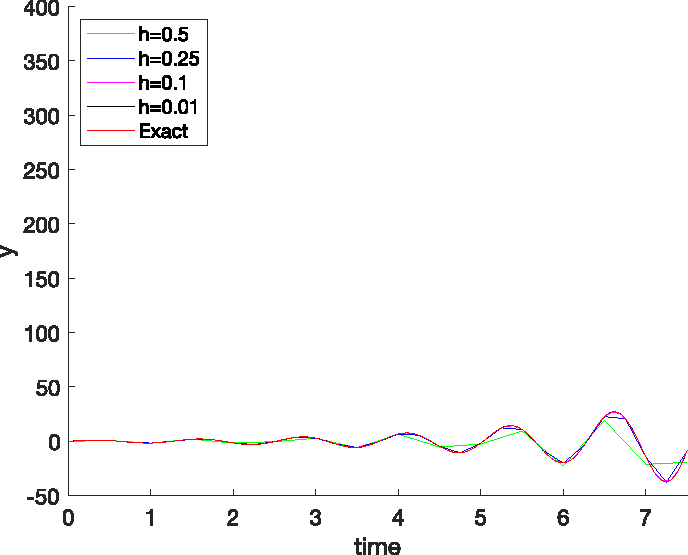
\includegraphics[scale=0.5]{files/example2Kutta.pdf}
    \caption{Results for smaller step sizes using RK4.}
    \label{fig:ex2kutta}
\end{figure}

\begin{exmp}
Solve the following initial value problem using RK4 method.
\begin{equation}
\begin{cases}
    y' = 10e^{-\frac{(t-2)^2}{2}}\left(10\cos(10t)-(t-2)\sin(10t)\right) &\\ y(0) = 0\quad t\in[0,7.5]&
\end{cases}
\end{equation}
\end{exmp}
As it was shown in previous sections, the exact solution is given by
\begin{equation}
    y(t) = 10e^{-\frac{(t-2)^2}{2}}\sin(10t)
\end{equation}


As the previous examples, table \ref{tab:ex3euler} and figure \ref{fig:ex3euler} show the numeric solution using different time steps.

\begin{table}[H]
\centering
\begin{tabular}{cccccc}
\hline
\textbf{Time}                          & \textbf{\boldmath$h=0.5$} & \textbf{\boldmath$h=0.25$} & \textbf{\boldmath$h=0.1$} & \textbf{\boldmath$h=0.01$} & \textbf{Exact} \\ \hline
\textbf{\boldmath$t=1$} & -3.5142                                  & 4.3668                                    & 2.2525                                   & -2.7473                                   & -3.2997        \\
\textbf{\boldmath$t=2$} & 14.5445                                  & -9.6097                                   & 1.4921                                   & 8.6760                                    & 9.1295         \\
\textbf{\boldmath$t=3$} & 1.8168                                   & 5.3571                                    & -4.4282                                  & -6.1167                                   & -5.9927        \\
\textbf{\boldmath$t=4$} & -4.4131                                  & -0.3869                                   & 1.5862                                   & 1.1155                                    & 1.0084         \\
\textbf{\boldmath$t=5$} & -0.2656                                  & -0.0688                                   & -0.1419                                  & -0.0409                                   & -0.0291        \\
\textbf{\boldmath$t=6$} & -0.7289                                  & 0.0268                                    & 0.0036                                   & -0.0007                                   & -0.0010        \\
\textbf{\boldmath$t=7$} & -0.7146                                  & 0.0194                                    & 0.0004                                   & 0.0000                                    & 0.0000         \\ \hline
\end{tabular}
\caption{Numerical results using RK4 method and different step sizes.}
\label{tab:ex3kutta}
\end{table}

\begin{figure}[H]
    \centering
    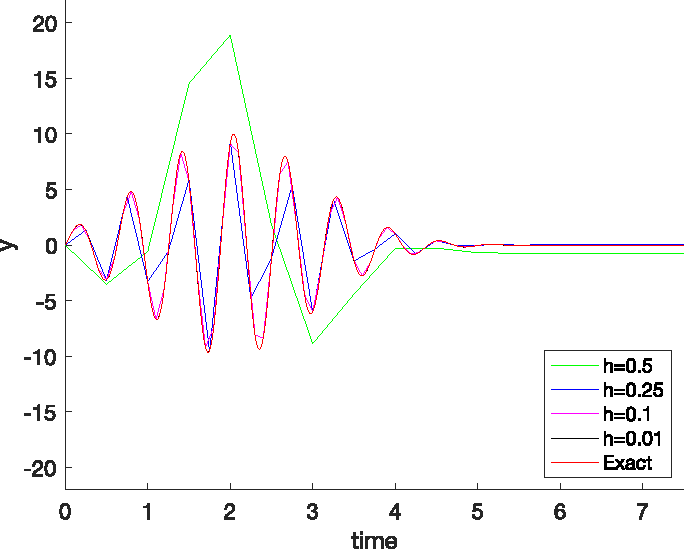
\includegraphics[scale=0.5]{files/example3Kutta.pdf}
    \caption{Plots for numerical approach.}
    \label{fig:ex3kutta}
\end{figure}

Notice than RK4 gives a significant improvement over the results obtained using Euler's method. Even for relatively large step sizes, the numeric approximation is bounded by the exact solution, and they stabilize closer to the exact solution, unlike Euler's method.
